\documentclass{beamer}
\usepackage[utf8]{inputenc}
\usepackage[spanish]{babel}
\usetheme{metropolis}           % Use metropolis theme
\graphicspath{{images/}}

\usepackage{multicol}
\usepackage{listings}
\usepackage[default]{sourcesanspro}

\usepackage[scale=2]{ccicons}

\usepackage[
    type={CC},
    modifier={by-nc-sa},
    version={4.0},
]{doclicense}



\hypersetup{
    colorlinks=true,
    linkcolor=black,
    filecolor=magenta,
    urlcolor=cyan,
}

\title{Cifrado MARS}


\date{\today}
\author{Antonio David Villegas Yeguas}
\institute{Universidad de Granada\\
\medskip
\textit{advy99@correo.ugr.es}
\doclicenseThis
}
\setbeamertemplate{caption}{\raggedright\insertcaption\par}

\begin{document}

 \maketitle

\begin{frame}{Índice}
\tableofcontents
\end{frame}




\section{Antecedentes}
\begin{frame}{Antecedentes}

	Uso generalizado de DES:

	\begin{itemize}
		\item Desarrollado por IBM.
		\item Red de Feistel.
		\item Tamaño de clave: 54 bits.
		\item Tamaño de bloque: 64 bits.
		\item Número de rondas: 16.
		\item Las S-Box no se llegaron a publicar durante mucho tiempo.
	\end{itemize}

\end{frame}


\section{AES process}
\begin{frame}{AES process}

	Torneo propuesto por el NIST para sustituir DES.

	Objetivos a cumplir para los participantes:

	\begin{itemize}
		\item Mayor tamaño de bloque, mínimo 128 bits.
		\item Longitud de claves mayor y variable, como mínimo de 128 bits.
		\item Implementación pública, incluidas S-boxes.
		\item Dominio público, para todos los S.O. y arquitecturas.
		\item Buena eficiencia tanto hardware como software.
	\end{itemize}

\end{frame}


\section{Sobre MARS}
\begin{frame}{Sobre MARS}

	Propuesta de IBM para el AES process.

	\begin{itemize}
		\item Parte del equipo de DES, como Don Coppersmith.
		\item Tamaño de bloque de 128 bits.
		\item Tamaño de clave variable, desde 128 hasta 448 bits.
		\item S-boxes publicadas en el paper de la propuesta.
	\end{itemize}


%\framebreak

\end{frame}

\section{Como funciona MARS}
\begin{frame}{Como funciona MARS: Redes de Feistel de tipo 3}

	Dado un texto plano dividido en cuatro partes $A_0$, $B_0$, $C_0$, $D_0$ y un entero $n$ de rondas, se realizan $n$ veces:

	\begin{enumerate}
		\item $D_{i + 1} = A_i$
		\item $F_1, F_2, F_3 = F(A_i, K_i)$
		\item $C_{i + 1} = D_i \oplus F_3$
		\item $B_{i + 1} = C_i \oplus F_2$
		\item $A_{i + 1} = B_i \oplus F_1$
	\end{enumerate}

%\framebreak

\end{frame}


\begin{frame}{Como funciona MARS: Operaciones internas}

	\begin{columns}[T]
		\begin{column}{.5\textwidth}
			Tres operaciones:

			\begin{enumerate}
				\item Mezcla directa: 8 rondas de transformaciones lineales.
				\item Núcleo criptográfico: 16 rondas de la red de Feistel de tipo 3.
				\item Deshacer mezcla directa: 8 rondas que invierten las transformaciones lineales iniciales.
			\end{enumerate}
		\end{column}
		\begin{column}{.5\textwidth}
			\begin{figure}[H]
				\centering
				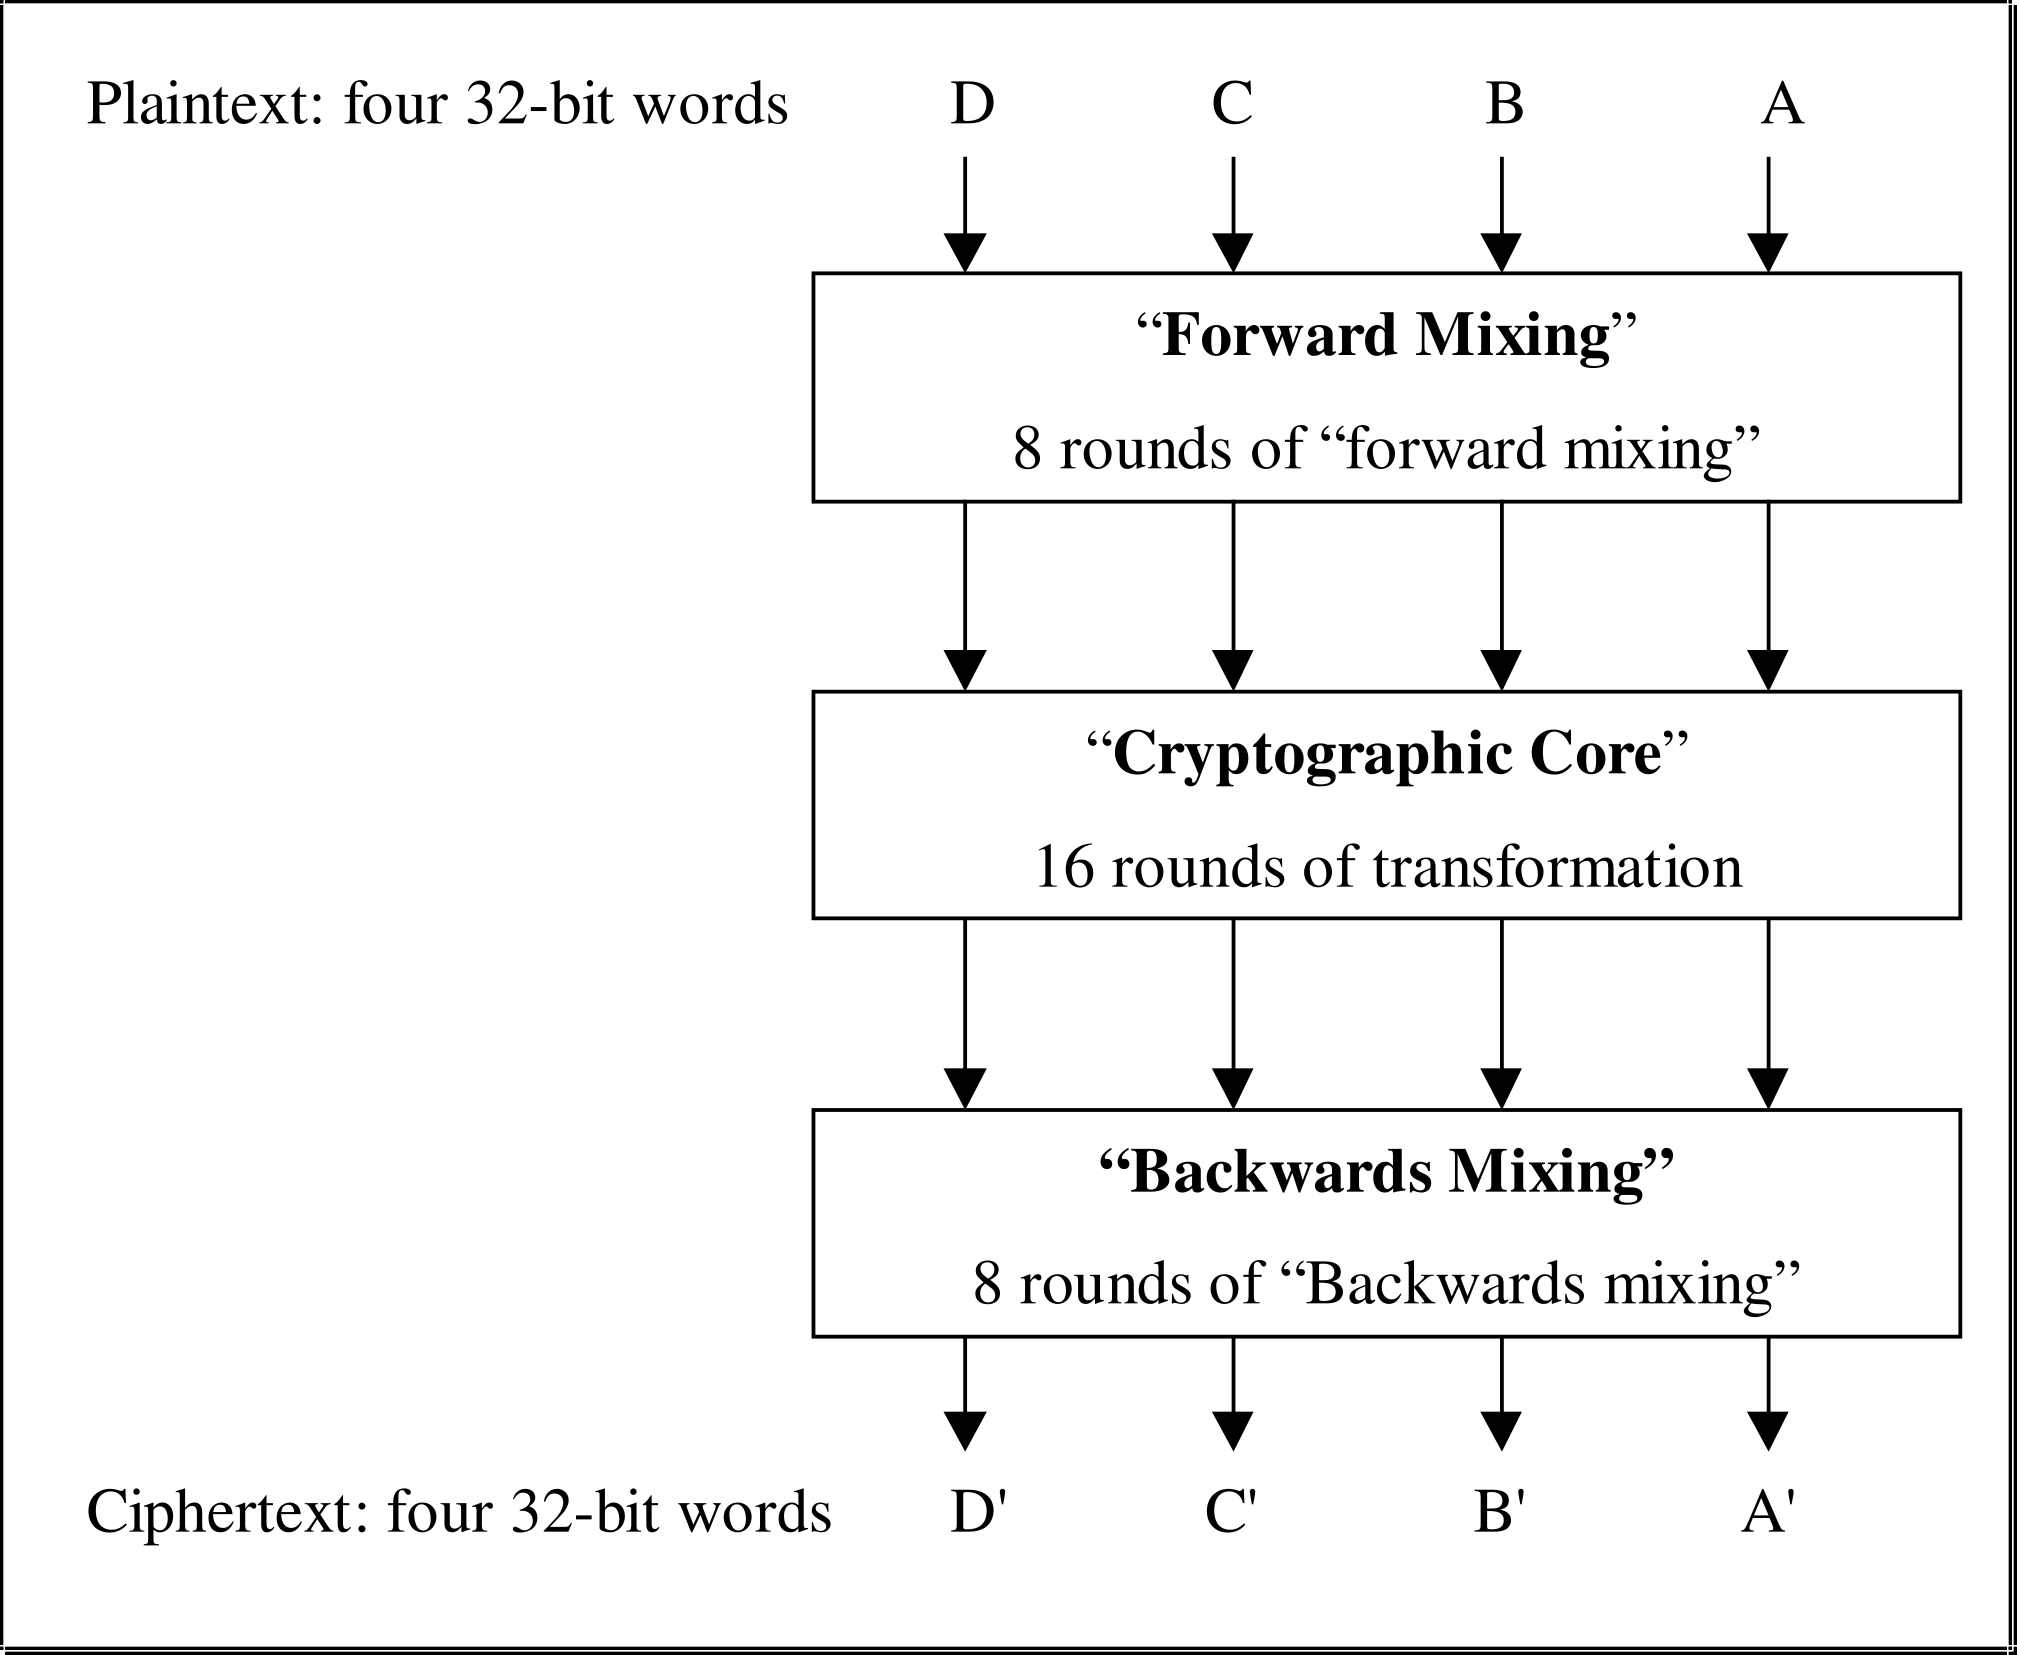
\includegraphics[scale = 0.5]{MARS.png}
				\caption{Estructura simplificada de MARS. Imagen obtenida de \cite{propuestaMARS}.} \label{fig:MARS}
			\end{figure}
		\end{column}

	\end{columns}

\end{frame}



\section{Problemas de MARS}
\begin{frame}[allowframebreaks]{Problemas de MARS}

	\begin{itemize}
		\item Demasiado lento.
		\item Demasiado complejo y poco elegante.

	\end{itemize}

%\framebreak

\end{frame}


\section{Prueba de MARS}
\begin{frame}[allowframebreaks]{Demostación: Crypto++}


%\framebreak

\end{frame}


\section{Bibliografía}
\begin{frame}[allowframebreaks]{Bibliografía}

\scriptsize
\begin{thebibliography}{9}

	\bibitem{propuestaMARS}

	Burnwick, C., \& Coppersmith, D. (1999). The Mars Encryption Algorithm. IBM, August, 27. \url{https://citeseerx.ist.psu.edu/viewdoc/download?doi=10.1.1.35.5887&rep=rep1&type=pdf}

	\bibitem{ampliacionPropuestaMARS}

	Burwick, C., Coppersmith, D., D’Avignon, E., Gennaro, R., Halevi, S., Jutla, C., ... \& Zunic, N. (1998). MARS-a candidate cipher for AES. NIST AES Proposal, 268, 80. \url{https://cryptosoft.de/docs/Mars.pdf}

	\bibitem{primerAES}

	Roback, E., \& Dworkin, M. (1999). First Advanced Encryption Standard (AES) Candidate Conference--Ventura, CA, August 20-22, 1998. Journal of Research of the National Institute of Standards and Technology, 104(1), 97. \url{https://nvlpubs.nist.gov/nistpubs/jres/104/1/j41ce-rob.pdf}

	\bibitem{primeraRondaAES}

	Nechvatal, J., Barker, E., Dodson, D., Dworkin, M., Foti, J., \& Roback, E. (1999). Status report on the first round of the development of the Advanced Encryption Standard. Journal of Research of the National Institute of Standards and Technology, 104(5), 435. \url{https://nvlpubs.nist.gov/nistpubs/jres/104/5/j45nec.pdf}

	\bibitem{comentariosAlgoritmosAES}
	Sybrandy, C., \& Macdonald, J. Public Comments Regarding The Advanced Encryption Standard (AES) Development Effort Round 2 Comments.	\url{https://csrc.nist.gov/CSRC/media/Projects/Cryptographic-Standards-and-Guidelines/documents/aes-development/R2comments.pdf}

	\bibitem{avanceAES}

	Nechvatal, J., Barker, E., Bassham, L., Burr, W., Dworkin, M., Foti, J., \& Roback, E. (2001). Report on the development of the Advanced Encryption Standard (AES). Journal of Research of the National Institute of Standards and Technology, 106(3), 511. \url{https://nvlpubs.nist.gov/nistpubs/jres/106/3/j63nec.pdf}

	\bibitem{impactoEconomicoAES}

	Leech, D. P., Ferris, S., \& Scott, J. T. (2019). The economic impacts of the advanced encryption standard, 1996–2017. Annals of Science and Technology Policy, 3(2), 142-257. \url{https://nvlpubs.nist.gov/nistpubs/gcr/2018/NIST.GCR.18-017.pdf}


	\bibitem{TFGOscar}

	Bermúdez Garrido, Óscar, \& Pedro Abelardo García Sánchez. Advanced Encryptation Standard Process.

\end{thebibliography}


\end{frame}

\section{Preguntas}


\end{document}
